\chapter{Reactie-enthalpieën}\label{ch:b2:reaction-enthalpy}

Een kampeergaspatroon, onder een kleine brander geschroefd: een paar gram
butaan brengen een liter water in enkele minuten aan de kook, en de blauwe
vlam onder de pan is veel heter dan het kokende water. Hoeveel warmte
geeft een reactie af, hoeveel daarvan bereikt de pan, en hoe heet kan de
vlam worden? Voor geen van deze vragen is een brander nodig: tabellen met
een paar getallen per stof, eens en voorgoed gemeten, geven de
reactiewarmte van elke reactie die met die stoffen te schrijven is, bij
elke temperatuur. Dit hoofdstuk bouwt die boekhouding op. Het past de
eerste hoofdwet van de thermodynamica, bekend uit de natuurkunde, toe op
een systeem waarvan de samenstelling verandert, definieert de
\omterm{def:b2:reaction-enthalpy:reaction-quantity}{reactie-enthalpie} als een partiële afgeleide, en laat zien hoe ze te
berekenen is uit vormingsenthalpieën, uit bindingsenthalpieën en langs
kringprocessen, hoe ze met de temperatuur verandert, en wat ze zegt over
vlammen en calorimeters.

\begin{recall}
Uit de natuurkunde: de eerste hoofdwet $\Delta U = W + Q$; de enthalpie $H = U + pV$,
een toestandsfunctie; bij constante uitwendige druk, tussen twee toestanden bij
die druk, is de opgenomen warmte $Q_p = \Delta H$; de warmtecapaciteit bij
constante druk $C_p = (\partial H/\partial T)_p$; de enthalpie van een
ideaal gas hangt alleen van $T$ af. Het deel van jaar~1 beschreef een reagerend
systeem met zijn voortgang $\xi$ en de stoichiometrische getallen $\nu_i$ van
$0 = \sum_i\nu_i\mathrm A_i$, en legde de standaardtoestand van elk deeltje vast
bij $p^\circ = \qty{1}{bar}$. Het schoolboek (jaar 11) noemde een reactie
\omterm{def:b2:reaction-enthalpy:exothermic}{exotherm} wanneer ze warmte afgeeft, en schatte verbrandingsenergieën uit
bindingsenergieën.
\end{recall}

\begin{omfigure}
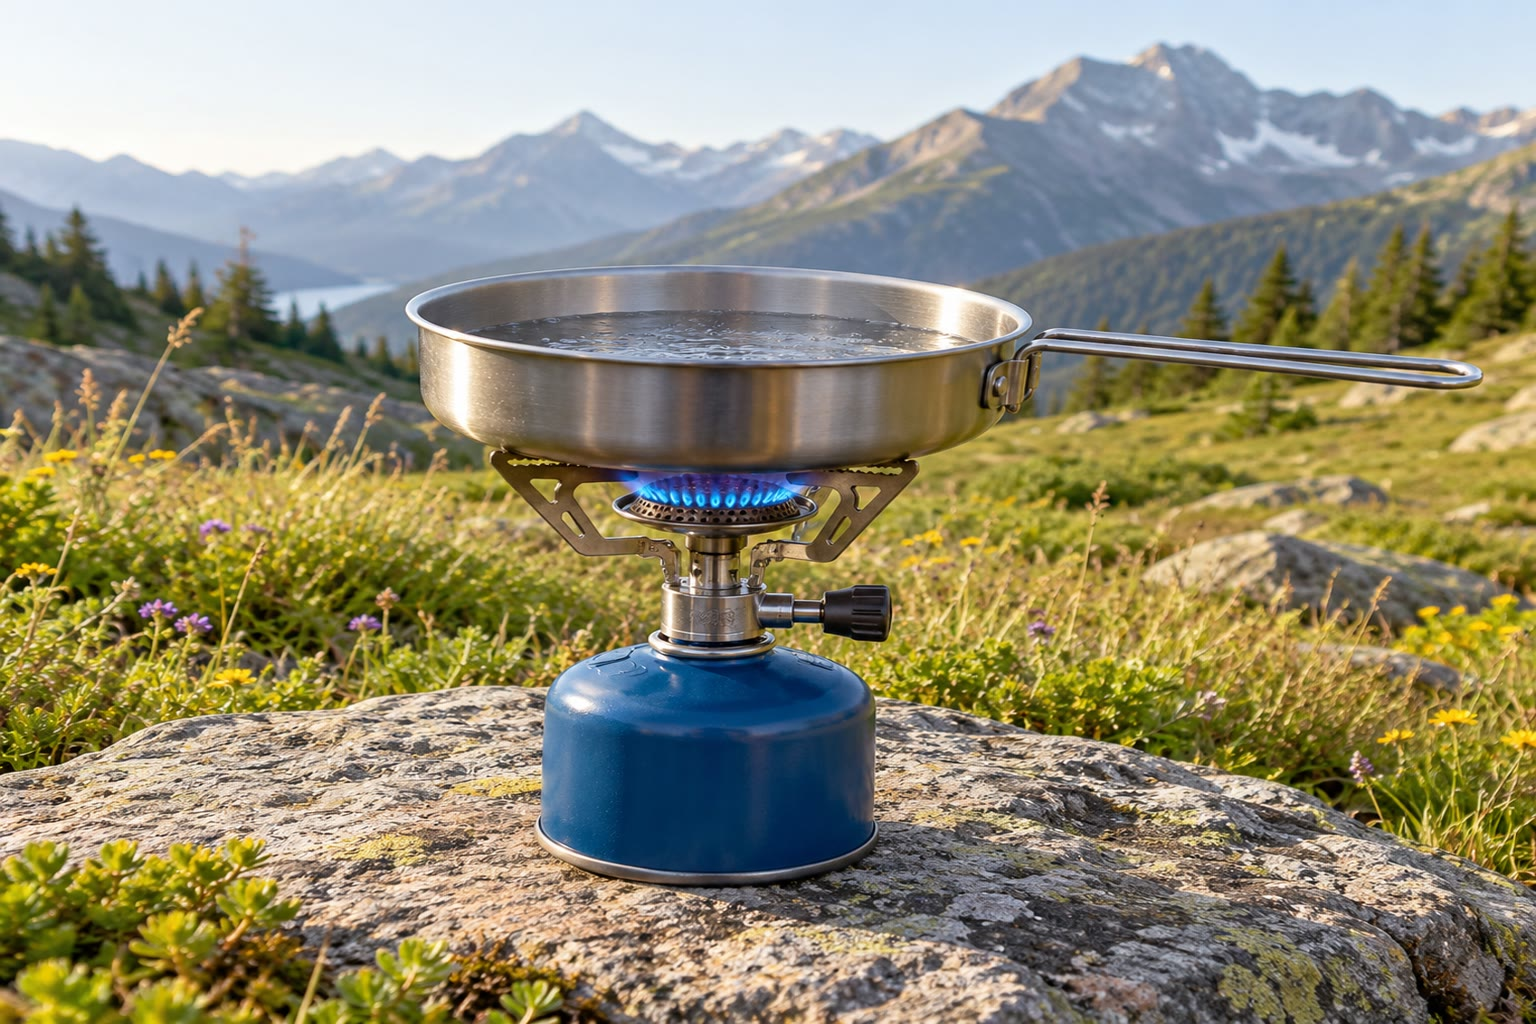
\includegraphics[width=0.6\linewidth]{images/book3/ai/b2-01-camping-stove.jpg}

{\small Een kampeerbrander: butaan uit het patroon verbrandt in de lucht onder
de pan. De warmte die per mol butaan vrijkomt, het deel dat het water
bereikt en de temperatuur van de vlam worden berekend in het
weekendprobleem van dit hoofdstuk.}
\end{omfigure}

\section{Reactiegrootheden}

Een gesloten systeem waarin de enige reactie $0 = \sum_i\nu_i\mathrm A_i$
plaatsvindt, wordt beschreven door zijn temperatuur, zijn druk en zijn voortgang:
de hoeveelheden zijn $n_i = n_{i,0} + \nu_i\xi$. Elke extensieve toestandsfunctie
van het systeem, bijvoorbeeld zijn enthalpie, is dan een functie $H(T, p,
\xi)$, met als totale differentiaal
\[
  \dd H = \left(\frac{\partial H}{\partial T}\right)_{p,\xi}\dd T
        + \left(\frac{\partial H}{\partial p}\right)_{T,\xi}\dd p
        + \left(\frac{\partial H}{\partial \xi}\right)_{T,p}\dd\xi .
\]

\begin{definition}[Reactiegrootheid, reactie-enthalpie]\label{def:b2:reaction-enthalpy:reaction-quantity}
Voor een extensieve toestandsfunctie $X$ van een gesloten systeem waarin de
reactie $0 = \sum_i\nu_i\mathrm A_i$ plaatsvindt, is de
\emph{reactiegrootheid}\index{reactiegrootheid} de partiële afgeleide
\[
  \Delta_r X = \left(\frac{\partial X}{\partial \xi}\right)_{T,p} ,
\]
de verandering van $X$ per eenheid voortgang bij vaste temperatuur en druk, in
eenheden van $X$ per mol. Voor $X = H$ is dat de
\emph{reactie-enthalpie}\index{reactie-enthalpie} $\Delta_r H$, in \unit{kJ/mol}.
\end{definition}

\begin{remark}[Een afgeleide, geen verschil]\label{rem:b2:reaction-enthalpy:operator}
Het symbool $\Delta_r$ is een operator: het werkt op de toestand van het
systeem, die het onveranderd laat. Wie de reactie anders schrijft
(alle coëfficiënten verdubbeld), verdubbelt $\Delta_r H$: een \omterm{def:b2:reaction-enthalpy:reaction-quantity}{reactiegrootheid}
heeft geen betekenis zonder haar reactievergelijking. Met de partiële molaire enthalpieën
$\bar H_i = (\partial H/\partial n_i)_{T,p,n_j}$ van de deeltjes
(\cref{ch:b2:chemical-potential}) geldt $\Delta_r H = \sum_i\nu_i\bar H_i$, volgens
de kettingregel toegepast op $n_i = n_{i,0} + \nu_i\xi$.
\end{remark}

\begin{proposition}[Opgenomen warmte bij constante temperatuur en druk]\label{prop:b2:reaction-enthalpy:qp}
Wanneer de reactie voortschrijdt van $\xi_1$ tot $\xi_2$ in een systeem dat op
constante $T$ en $p$ gehouden wordt, neemt het systeem de warmte
\[
  Q_p = \int_{\xi_1}^{\xi_2}\Delta_r H\,\dd\xi = \Delta_r H\,(\xi_2 - \xi_1)
\]
op, als $\Delta_r H$ niet van $\xi$ afhangt.
\end{proposition}

\begin{proof}
Bij constante $p$ (en hier constante uitwendige druk) is de opgenomen warmte
de verandering van de enthalpie, $Q_p = \Delta H$ (natuurkunde). Bij vaste $T$ en $p$
reduceert de differentiaal van $H$ tot $\dd H = \Delta_r H\,\dd\xi$; integreren
van $\xi_1$ tot $\xi_2$ geeft het resultaat.
\end{proof}

\begin{definition}[Exotherm, endotherm, atherm]\label{def:b2:reaction-enthalpy:exothermic}
Een reactie is \emph{exotherm}\index{exotherm} in een gegeven toestand als
$\Delta_r H < 0$: voorwaarts verlopend bij constante $T$ en $p$ geeft ze warmte af aan de
omgeving. Ze is \emph{endotherm}\index{endotherm} als $\Delta_r H >
0$, en \emph{atherm}\index{atherm} als $\Delta_r H = 0$.
\end{definition}

De reactiewarmte hangt in het algemeen niet af van de samenstelling:
voor ideale gassen en voor zuivere vaste stoffen en vloeistoffen hangt de enthalpie van elk
deeltje niet af van wat het omringt, en ligt $\Delta_r H$ vast
zodra $T$ vastligt.

\begin{proposition}[Ideale systemen]\label{prop:b2:reaction-enthalpy:ideal}
In een mengsel van ideale gassen met zuivere gecondenseerde fasen hangt $\Delta_r H$
alleen van de temperatuur af, en is het gelijk aan de \omterm{def:b2:reaction-enthalpy:standard-reaction-enthalpy}{standaardreactie-enthalpie}
$\Delta_r H^\circ(T)$ die hieronder gedefinieerd wordt. Voor opgeloste stoffen in verdunde
oplossing geldt de gelijkheid bij goede benadering.
\end{proposition}

\begin{proof}
In een mengsel van ideale gassen gedraagt elk gas zich alsof het alleen is, met een enthalpie
$n_iH_{m,i}(T)$ die niet van $p$ afhangt (natuurkunde: de enthalpie van een
ideaal gas hangt alleen van $T$ af). Een zuivere vaste stof of vloeistof heeft $H = n_iH_{m,i}(T,
p)$, en $(\partial H_m/\partial p)_T = V_m(1 - \alpha T)$ bedraagt enkele
\unit{J/(mol.bar)} voor een gecondenseerde fase, verwaarloosbaar naast reactie-enthalpieën
van tientallen \unit{kJ/mol}. Dus $H = \sum_in_iH_{m,i}(T)$, waarvan de
afgeleide naar $\xi$ gelijk is aan $\sum_i\nu_iH_{m,i}(T)$: die hangt alleen van
$T$ af, en de waarde ervan is die welke berekend wordt met elk deeltje in zijn
standaardtoestand.
\end{proof}

\section{Standaardreactie-enthalpieën en de wet van Hess}

\begin{definition}[Standaardreactiegrootheid]\label{def:b2:reaction-enthalpy:standard-reaction-enthalpy}
De \emph{standaardreactiegrootheid}\index{standaardreactiegrootheid}
$\Delta_r X^\circ(T) = \sum_i\nu_iX_{m,i}^\circ(T)$ is de \omterm{def:b2:reaction-enthalpy:reaction-quantity}{reactiegrootheid}
berekend met elk deeltje in zijn standaardtoestand bij temperatuur $T$, waarbij de
$X_{m,i}^\circ$ de molaire standaardwaarden zijn. Voor $X = H$ is dat de
\emph{standaardreactie-enthalpie}\index{standaardreactie-enthalpie}
$\Delta_r H^\circ(T)$; ze hangt alleen van $T$ af.
\end{definition}

Alleen enthalpieverschillen zijn meetbaar; daarom wordt eens en voorgoed een
referentie gekozen, zoals de waterstofelektrode gekozen werd voor potentialen.

\begin{definition}[Standaardreferentietoestand, standaardvormingsenthalpie]\label{def:b2:reaction-enthalpy:formation}
De \emph{standaardreferentietoestand}\index{standaardreferentietoestand} van een
element bij temperatuur $T$ is zijn stabielste vorm bij $T$ onder $p^\circ$:
\ce{H2}, \ce{O2}, \ce{N2} en \ce{Cl2} als ideale gassen, koolstof als
grafiet, natrium als metaal, broom als vloeistof (bij \qty{298}{K}).
De \emph{standaardvormingsenthalpie}\index{standaardvormingsenthalpie}
$\Delta_f H^\circ$ van een verbinding is de \omterm{def:b2:reaction-enthalpy:standard-reaction-enthalpy}{standaardreactie-enthalpie}
van haar vormingsreactie, de reactie die één mol van de
verbinding maakt uit haar elementen in hun referentietoestand. Per constructie
is $\Delta_f H^\circ = 0$ voor een element in zijn referentietoestand.
\end{definition}

\begin{example}[Vormingsreacties]\label{ex:b2:reaction-enthalpy:formation}
De vormingsreactie van water is \ce{H2(g) + 1/2O2(g) -> H2O(l)}, met
$\Delta_f H^\circ = \qty{-285.83}{kJ/mol}$ bij \qty{298.15}{K}; die van
methaan is \ce{C(s) + 2H2(g) -> CH4(g)}, $\Delta_f H^\circ =
\qty{-74.9}{kJ/mol}$; die van stikstofmonoxide, \ce{1/2N2(g) + 1/2O2(g) ->
NO(g)}, $\Delta_f H^\circ = \qty{+90.3}{kJ/mol}$: een \omterm{def:b2:reaction-enthalpy:exothermic}{endotherme} verbinding,
die de hete gassen van een motor toch vormen. De halve coëfficiënten
zijn geen probleem: de vormingsreactie is een boekhoudkundig hulpmiddel, geen
mechanisme.
% ledger: dfh:H2O-l, dfh:CH4_g, dfh:NO_g
\end{example}

\begin{theorem}[Wet van Hess]\label{thm:b2:reaction-enthalpy:hess}
Als een reactie de som is, met coëfficiënten $\lambda_k$, van reacties $k$,
dan is haar \omterm{def:b2:reaction-enthalpy:standard-reaction-enthalpy}{standaardreactie-enthalpie} dezelfde combinatie van die van hen:
$\Delta_r H^\circ = \sum_k\lambda_k\Delta_r H_k^\circ$
(\emph{wet van Hess}\index{wet van Hess}). In het bijzonder kan een \omterm{def:b2:reaction-enthalpy:standard-reaction-enthalpy}{standaardreactie-enthalpie}
berekend worden langs elke weg van reacties die van de
beginstoffen naar de reactieproducten leidt.
\end{theorem}

\begin{proof}
Elke $\Delta_r H_k^\circ = \sum_i\nu_{i,k}H_{m,i}^\circ$ is lineair in de
stoichiometrische getallen. Als de reactie $\sum_k\lambda_k$ maal de
reacties $k$ is, zijn haar stoichiometrische getallen $\nu_i = \sum_k\lambda_k
\nu_{i,k}$, en $\Delta_r H^\circ = \sum_i\nu_iH_{m,i}^\circ = \sum_k\lambda_k
\sum_i\nu_{i,k}H_{m,i}^\circ$. Achter de algebra zit de eerste hoofdwet: $H$ is een
toestandsfunctie, dus haar verandering tussen dezelfde begin- en eindtoestand
hangt niet af van de gevolgde weg.
\end{proof}

\begin{proposition}[Reactie-enthalpie uit vormingsenthalpieën]\label{prop:b2:reaction-enthalpy:formation-sum}
$\Delta_r H^\circ(T) = \sum_i\nu_i\,\Delta_f H_i^\circ(T)$.
\end{proposition}

\begin{proof}
Neem de weg die de beginstoffen ontleedt in hun elementen in hun
referentietoestand (het omgekeerde van hun vormingsreacties, met de
coëfficiënten $-\nu_i > 0$), en daarna de reactieproducten vormt uit dezelfde elementen
(coëfficiënten $\nu_i > 0$). De elementen vallen tegen elkaar weg omdat de vergelijking
klopt, en de \omterm{thm:b2:reaction-enthalpy:hess}{wet van Hess} telt de enthalpieën op.
\end{proof}

\begin{omfigure}
\begin{tikzpicture}[font=\small, >={Stealth}, y=0.0062cm]
  \draw[->] (0,-1000) -- (0,180) node[above] {$H^\circ$ (\unit{kJ/mol})};
  \foreach \y in {0,-200,-400,-600,-800,-1000} \draw (-0.08,\y) -- (0.08,\y) node[left=4pt] {$\y$};
  % levels
  \draw[very thick] (1.0,0) -- (4.6,0) node[right] {\ce{C(s) + 2H2(g) + 2O2(g)}};
  \draw[very thick, omDef] (1.0,-74.9) -- (4.6,-74.9);
  \node[right, omDef] at (4.6,-110) {\ce{CH4(g) + 2O2(g)}};
  \draw[very thick, omThm] (1.0,-965.2) -- (4.6,-965.2) node[right] {\ce{CO2(g) + 2H2O(l)}};
  % arrows
  \draw[->, omDef, thick] (1.6,0) -- (1.6,-74.9);
  \node[omDef, anchor=south west, font=\footnotesize] at (1.1,5) {$\Delta_f H^\circ(\ce{CH4}) = -74.9$};
  \draw[->, omThm, thick] (3.9,0) -- (3.9,-965.2);
  \node[right, omThm, align=left] at (3.95,-500) {$\Delta_f H^\circ(\ce{CO2})$\\ $+ 2\Delta_f H^\circ(\ce{H2O})$\\ $= -965.2$};
  \draw[->, thick] (2.75,-74.9) -- (2.75,-965.2);
  \node[left, align=right] at (2.7,-650) {$\Delta_r H^\circ$\\ $= -890.3$};
\end{tikzpicture}

{\small Enthalpieniveaus voor de verbranding van methaan bij \qty{298.15}{K}.
De elementen in hun referentietoestand vormen het nulpunt. Methaan ligt
\qty{74.9}{kJ/mol} lager, de reactieproducten \qty{965.2}{kJ/mol} lager:
de verbrandingsenthalpie is het verschil, \qty{-890.3}{kJ/mol}, welke
weg de vlam ook werkelijk volgt.}
% ledger: dfh:CH4_g, dfh:CO2, dfh:H2O-l
\end{omfigure}

\begin{example}[Verbranding van methaan]\label{ex:b2:reaction-enthalpy:methane}
Voor \ce{CH4(g) + 2O2(g) -> CO2(g) + 2H2O(l)} is
$\Delta_r H^\circ = -393.51 + 2(-285.83) - (-74.87) - 0 =
\qty{-890.3}{kJ/mol}$ bij \qty{298.15}{K}. De waarde gemeten in een
calorimeter is \qty{-890.7}{kJ/mol}: tabel en vlam komen overeen binnen
de onzekerheid van de gegevens. Als het water als damp vertrekt
($\Delta_f H^\circ = \qty{-241.83}{kJ/mol}$), is $\Delta_r H^\circ =
\qty{-802.3}{kJ/mol}$: het verschil, \qty{88.0}{kJ}, is de verdampingsenthalpie
van twee mol water, die een condensatieketel terugwint door
zijn rookgassen te condenseren.
% ledger: dfh:CO2, dfh:H2O-l, dfh:CH4_g, dch:CH4, dfh:H2O_g (computed in figdata/bachelor-2/thermo-data.py)
\end{example}

\begin{method}[Een kringproces van Hess]\label{met:b2:reaction-enthalpy:hess-cycle}
Zo vind je de enthalpie van een reactie die niet rechtstreeks meetbaar is:
\begin{enumerate}
  \item schrijf de doelreactie op, met de aggregatietoestanden;
  \item zoek reacties met bekende enthalpie (verbrandingen, vormingsreacties) waarvan de
        combinatie, met coëfficiënten $\lambda_k$, de doelreactie oplevert;
  \item controleer dat elk deeltje dat niet in de doelreactie voorkomt, wegvalt;
  \item tel de enthalpieën op met dezelfde coëfficiënten.
\end{enumerate}
\end{method}

\begin{example}[Van koolstof naar koolstofmonoxide]\label{ex:b2:reaction-enthalpy:co}
Bij het verbranden van koolstof ontstaat altijd wat koolstofdioxide; daarom wordt de enthalpie van
\ce{C(s) + 1/2O2(g) -> CO(g)} niet rechtstreeks gemeten. De twee verbrandingen
\ce{C(s) + O2(g) -> CO2(g)} ($\qty{-393.51}{kJ/mol}$) en \ce{CO(g) +
1/2O2(g) -> CO2(g)} ($\qty{-283.0}{kJ/mol}$, gemeten) zijn dat wel; de doelreactie is
de eerste min de tweede: $\Delta_r H^\circ = -393.51 + 283.0 =
\qty{-110.5}{kJ/mol}$, de vormingsenthalpie van koolstofmonoxide.
% ledger: dfh:CO2, dfh:CO_g
\end{example}

\begin{history}[Germain Henri Hess]
\begin{minipage}[t]{0.2\linewidth}\vspace{0pt}
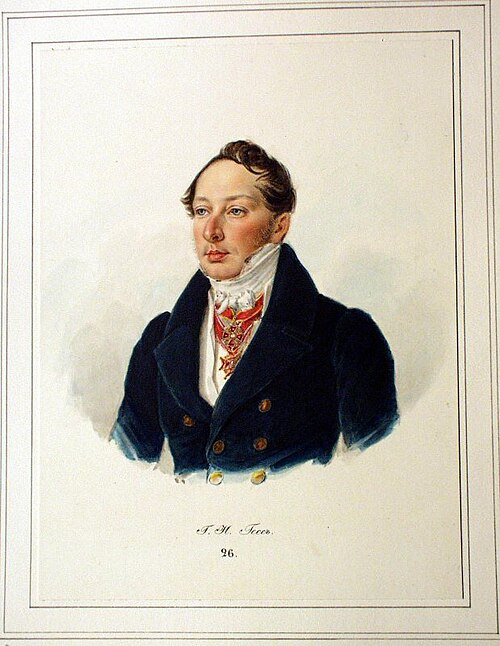
\includegraphics[width=\linewidth]{images/book3/hess.jpg}
\end{minipage}\hfill
\begin{minipage}[t]{0.76\linewidth}\vspace{0pt}
Germain Henri Hess (1802--1850), hoogleraar scheikunde in Sint-Petersburg,
mat de warmte die vrijkomt wanneer zwavelzuur in verscheidene stappen verdund of
geneutraliseerd wordt, en vond in 1840 dat het totaal niet afhing
van de gevolgde stappen: de ``wet van de constante warmtesom'', geformuleerd
nog vóór de eerste hoofdwet van de thermodynamica zelf, die haar verklaart.
(Portret door I. I. Reimers, 1837--1838; CC BY-SA 4.0, Wikimedia Commons.)
\end{minipage}
\end{history}

\section{Reactie-enthalpieën berekenen}

\subsection*{Uit bindingsenthalpieën}

Wanneer de vormingsenthalpie van een verbinding ontbreekt, levert de energie van haar
bindingen een schatting, in de gasfase.

\begin{definition}[Bindingsdissociatie-enthalpie, gemiddelde bindingsenthalpie]\label{def:b2:reaction-enthalpy:bond-enthalpy}
De \emph{bindingsdissociatie-enthalpie}\index{bindingsdissociatie-enthalpie} van
een binding A--B in een gasvormig molecuul is de \omterm{def:b2:reaction-enthalpy:standard-reaction-enthalpy}{standaardreactie-enthalpie} van het
verbreken van die binding tot twee gasvormige fragmenten, \ce{AB(g) -> A(g) + B(g)}
voor een tweeatomig molecuul. Wanneer een molecuul $n$ gelijke bindingen heeft, is zijn
\emph{gemiddelde bindingsenthalpie}\index{gemiddelde bindingsenthalpie} de standaardenthalpie
van zijn volledige atomisering tot gasvormige atomen, gedeeld door $n$.
\end{definition}

De atomiseringsenthalpieën zijn zelf vormingsenthalpieën: die van
de gasvormige atomen, min die van het molecuul. De onderstaande tabel is
op die manier berekend.

\begin{omfigure}
\begin{tabular}{lrl}
\hline
binding & enthalpie (\unit{kJ/mol}) & verkregen uit \\
\hline
H--H & 436 & \ce{H2}, dissociatie \\
O=O & 498 & \ce{O2}, dissociatie \\
N$\equiv$N & 945 & \ce{N2}, dissociatie \\
Cl--Cl & 243 & \ce{Cl2}, dissociatie \\
H--Cl & 432 & \ce{HCl}, dissociatie \\
C--H & 416 & \ce{CH4}, gemiddelde van vier \\
N--H & 391 & \ce{NH3}, gemiddelde van drie \\
O--H & 464 & \ce{H2O}, gemiddelde van twee \\
C=O & 804 & \ce{CO2}, gemiddelde van twee \\
C--C & 330 & \ce{C2H6}, met C--H uit methaan \\
C=C & 589 & \ce{C2H4}, met C--H uit methaan \\
\hline
\end{tabular}

\smallskip
{\small Bindingsenthalpieën bij \qty{298.15}{K}, berekend uit de
standaardvormingsenthalpieën van de gasvormige atomen en moleculen. De laatste twee
regels tonen de grens van de methode: een C--H-binding van ethaan is niet precies
die van methaan, en de waarde voor C--C erft het verschil.}
% ledger: dfh:C_g, janaf:H, dfh:O_g, dfh:N_g, janaf:Cl, janaf:HCl, dfh:CH4_g, dfh:NH3_g, dfh:H2O_g, dfh:CO2, dfh:C2H6_g, dfh:C2H4_g (computed in figdata/bachelor-2/thermo-data.py)
\end{omfigure}

\begin{proposition}[Schatting uit bindingsenthalpieën]\label{prop:b2:reaction-enthalpy:bond-estimate}
Voor een reactie tussen gassen geldt
\[
  \Delta_r H^\circ \approx \sum(\text{enthalpieën verbroken bindingen}) -
  \sum(\text{enthalpieën gevormde bindingen}).
\]
\end{proposition}

\begin{proof}
Volg de weg die elke beginstof atomiseert (enthalpie: de verbroken bindingen)
en daarna de reactieproducten uit de atomen opbouwt (min de gevormde bindingen). De \omterm{thm:b2:reaction-enthalpy:hess}{wet van Hess}
maakt de som exact wanneer elke bindingsenthalpie die van de binding in haar
eigen molecuul is; die vervangen door een gemiddelde waarde uit een ander molecuul is de
benadering.
\end{proof}

\begin{example}[Hydrogenering van etheen]\label{ex:b2:reaction-enthalpy:hydrogenation}
In \ce{C2H4(g) + H2(g) -> C2H6(g)} worden één C=C en één H--H verbroken en
vervangen door één C--C en twee C--H. Met de tabel: $589 + 436 - 330 - 2
\times 416 = \qty{-137}{kJ/mol}$; uit vormingsenthalpieën is de waarde
\qty{-136.3}{kJ/mol}. De overeenkomst is hier goed omdat de C--C en C=C van de tabel
uit precies deze moleculen verkregen zijn; voor een molecuul dat niet lijkt op
die van de tabel is een fout van 10 tot \qty{30}{kJ/mol} gewoon.
% ledger: dfh:C2H4_g, dfh:C2H6_g
\end{example}

\subsection*{Roosterenthalpieën: het kringproces van Born--Haber}

\begin{definition}[Roosterenthalpie]\label{def:b2:reaction-enthalpy:lattice-enthalpy}
De \emph{roosterenthalpie}\index{roosterenthalpie} van een ionkristal is
de \omterm{def:b2:reaction-enthalpy:standard-reaction-enthalpy}{standaardreactie-enthalpie} van zijn dissociatie tot gasvormige ionen: voor
natriumchloride \ce{NaCl(s) -> Na+(g) + Cl-(g)}. Ze is positief, en
meet de cohesie van het kristal.
\end{definition}

Ze is niet rechtstreeks meetbaar, maar een kringproces via de elementen levert haar
uit meetbare grootheden: de vormingsenthalpie van het kristal, de
atomisering van de elementen, de ionisatie-energie van het metaal en de
elektronenaffiniteit van het niet-metaal (beide gedefinieerd in het deel van jaar~1).

\begin{omfigure}
\begin{tikzpicture}[font=\small, >={Stealth}, y=0.0058cm]
  \def\lw{5.0}
  % levels (kJ/mol relative to Na(s) + 1/2 Cl2(g))
  \draw[thick] (0,0) -- (\lw,0) node[right] {\ce{Na(s) + 1/2Cl2(g)}};
  \draw[thick] (0,107.5) -- (\lw,107.5) node[right] {\ce{Na(g) + 1/2Cl2(g)}};
  \draw[thick] (0,228.8) -- (\lw,228.8) node[right] {\ce{Na(g) + Cl(g)}};
  \draw[thick] (0,724.6) -- (\lw,724.6) node[right] {\ce{Na+(g) + e- + Cl(g)}};
  \draw[thick] (0,376.1) -- (\lw,376.1) node[right] {\ce{Na+(g) + Cl-(g)}};
  \draw[thick] (0,-411.1) -- (\lw,-411.1) node[right] {\ce{NaCl(s)}};
  % the path through the elements, on the left
  \draw[->, omDef] (0.4,0) -- (0.4,107.5);
  \node[omDef, left, font=\footnotesize] at (0.35,53) {sublimatie $107.5$};
  \draw[->, omDef] (0.4,107.5) -- (0.4,228.8);
  \node[omDef, left, font=\footnotesize] at (0.35,168) {$\tfrac12$ dissociatie $121.3$};
  \draw[->, omDef] (0.4,228.8) -- (0.4,724.6);
  \node[omDef, left, font=\footnotesize] at (0.35,480) {ionisatie van Na $495.8$};
  \draw[->, omThm] (1.4,724.6) -- (1.4,376.1);
  \node[omThm, right, font=\footnotesize] at (1.45,560) {elektronenopname $-348.6$};
  \draw[->, omProp] (2.3,0) -- (2.3,-411.1);
  \node[omProp, left, font=\footnotesize] at (2.25,-205) {vorming $-411.1$};
  % the lattice enthalpy, the only unknown
  \draw[->, thick] (3.6,-411.1) -- (3.6,376.1);
  \node[right, font=\footnotesize] at (3.65,-205) {roosterenthalpie $787$};
\end{tikzpicture}

{\small Het kringproces van Born--Haber voor natriumchloride bij \qty{298}{K}
(\unit{kJ/mol}). Van het kristal omhoog naar de gasvormige ionen via de
\omterm{def:b2:reaction-enthalpy:lattice-enthalpy}{roosterenthalpie}, of de omweg via de elementen: beide leiden tot hetzelfde niveau. De
\omterm{def:b2:reaction-enthalpy:lattice-enthalpy}{roosterenthalpie} is de enige onbekende van het kringproces.}
% ledger: dfh:NaCl_cr, dfh:Na_g, janaf:Cl, ie:Na, ea:Cl
\end{omfigure}

\begin{method}[Het kringproces van Born--Haber]\label{met:b2:reaction-enthalpy:born-haber}
\begin{enumerate}
  \item Teken vanuit de elementen in hun referentietoestand twee wegen: een
        naar het kristal (vorming), een naar de gasvormige ionen (sublimatie van
        het metaal, atomisering van het niet-metaal, ionisatie, elektronenopname).
  \item Sluit het kringproces met de \omterm{def:b2:reaction-enthalpy:lattice-enthalpy}{roosterenthalpie}, van het kristal omhoog naar
        de gasvormige ionen.
  \item Schrijf op dat de som van de enthalpieën rond het kringproces nul is, en
        los op naar de onbekende. Ionisatie-energieën en elektronenaffiniteiten
        staan in tabellen in eV per atoom: vermenigvuldig met $N_A e = \qty{96.485}{kJ/(mol.eV)}$.
\end{enumerate}
\end{method}

\begin{example}[Natriumchloride]\label{ex:b2:reaction-enthalpy:nacl}
$\Delta_{\text{lat}}H^\circ = 411.1 + 107.5 + 121.3 + 495.8 - 348.6 =
\qty{787}{kJ/mol}$. De ionisatie-energie en de elektronenaffiniteit zijn
energieën bij \qty{0}{K}; hun correcties naar \qty{298}{K} ($+\tfrac52RT$
voor elk) heffen elkaar op tussen de twee stappen. Een kristalmodel met puntladingen
geeft een vergelijkbare waarde; daarom heet natriumchloride ionisch.
% ledger: dfh:NaCl_cr, dfh:Na_g, janaf:Cl, ie:Na, ea:Cl (computed in figdata/bachelor-2/thermo-data.py)
\end{example}

\section{Reactie-enthalpieën en temperatuur}

Tabellen geven $\Delta_f H^\circ$ bij \qty{298.15}{K}. Een reactor werkt bij
\qty{700}{K}, een vlam bij \qty{2000}{K}: hoe verandert $\Delta_r H^\circ$
met de temperatuur?

\begin{theorem}[Wet van Kirchhoff]\label{thm:b2:reaction-enthalpy:kirchhoff}
\[
  \frac{\dd\Delta_r H^\circ}{\dd T} = \Delta_r C_p^\circ =
  \sum_i\nu_i C_{p,m,i}^\circ ,
\]
zodat $\Delta_r H^\circ(T_2) = \Delta_r H^\circ(T_1) + \int_{T_1}^{T_2}
\Delta_r C_p^\circ\,\dd T$ (\emph{wet van Kirchhoff}\index{wet van Kirchhoff}),
zolang er tussen $T_1$ en $T_2$ geen faseovergang optreedt.
\end{theorem}

\begin{proof}
Met elk deeltje in zijn standaardtoestand is $H^\circ(T, \xi) = \sum_in_i
H^\circ_{m,i}(T)$ een functie van twee variabelen waarvan de tweede partiële
afgeleiden continu zijn; volgens de stelling van Schwarz mogen ze verwisseld worden:
\[
  \frac{\dd\Delta_r H^\circ}{\dd T} = \frac{\partial}{\partial T}
  \frac{\partial H^\circ}{\partial\xi} = \frac{\partial}{\partial\xi}
  \frac{\partial H^\circ}{\partial T} = \frac{\partial}{\partial\xi}
  \sum_in_iC^\circ_{p,m,i} = \sum_i\nu_iC^\circ_{p,m,i}.
\]
Integreren tussen $T_1$ en $T_2$ geeft de tweede vorm. Een faseovergang
van een deeltje binnen het interval voegt zijn overgangsenthalpie toe,
met het stoichiometrisch getal als factor.
\end{proof}

\begin{example}[Ammoniaksynthese bij hoge temperatuur]\label{ex:b2:reaction-enthalpy:kirchhoff}
Voor \ce{N2(g) + 3H2(g) -> 2NH3(g)} is $\Delta_r H^\circ(298) =
\qty{-91.9}{kJ/mol}$ en, met de warmtecapaciteiten bij \qty{298}{K},
$\Delta_r C_p^\circ = 2(35.65) - 29.12 - 3(28.84) =
\qty{-44.3}{J/(K.mol)}$. Constant verondersteld geeft dat $\Delta_r
H^\circ(700) = -91.9 - 0.0443 \times 402 = \qty{-109.7}{kJ/mol}$. De tabellen,
die de warmtecapaciteiten volgen terwijl die met de temperatuur toenemen, geven
\qty{-105.2}{kJ/mol}: de schatting met constante $C_p$ zit er 4\,\% naast, een
redelijke prijs voor een berekening van één regel. Over \qty{400}{K} verandert de
\omterm{def:b2:reaction-enthalpy:reaction-quantity}{reactie-enthalpie} met ongeveer een zevende.
% ledger: dfh:NH3_g, cp:NH3_g.298, cp:N2_g.298, cp:H2_g.298, janafdfH:NH3.700 (computed in figdata/bachelor-2/thermo-data.py)
\end{example}

\section{Adiabatische reacties en calorimetrie}

\subsection*{Vlamtemperatuur}

In een vlam verloopt de reactie snel en heeft de warmte geen tijd om weg te gaan: de
gassen verhitten zichzelf.

\begin{definition}[Adiabatische vlamtemperatuur]\label{def:b2:reaction-enthalpy:flame-temperature}
De \emph{adiabatische vlamtemperatuur}\index{adiabatische vlamtemperatuur}
van een brandstof is de temperatuur die de producten van haar volledige
verbranding bereiken wanneer de reactie bij constante druk plaatsvindt, zonder
enige warmte-uitwisseling, uitgaande van beginstoffen bij \qty{298}{K}.
\end{definition}

\begin{proposition}[Een vlamtemperatuur berekenen]\label{prop:b2:reaction-enthalpy:flame}
Als de reactie met $\xi$ voortschrijdt vanuit beginstoffen bij $T_0$ en het eindsysteem
warmtecapaciteit $C_p(T)$ heeft, voldoet de eindtemperatuur $T_f$ aan
\[
  \xi\,\Delta_r H^\circ(T_0) + \int_{T_0}^{T_f}C_p(T)\,\dd T = 0 .
\]
\end{proposition}

\begin{proof}
Adiabatisch en bij constante druk heeft de transformatie $\Delta H =
Q_p = 0$. Omdat $H$ een toestandsfunctie is, geeft elke weg tussen dezelfde begin- en
eindtoestand dezelfde $\Delta H$. Neem de weg van
de figuur hieronder: eerst de reactie bij $T_0$, met
$\Delta H_1 = \xi\Delta_r H^\circ(T_0)$ (\cref{prop:b2:reaction-enthalpy:qp},
bij ideaal gedrag); daarna het opwarmen van het eindsysteem van $T_0$ tot
$T_f$, $\Delta H_2 = \int C_p\,\dd T$. Hun som is nul.
\end{proof}

\begin{omfigure}
\begin{tikzpicture}[font=\small, >={Stealth}]
  \draw[->] (0,0) -- (6.2,0) node[right] {voortgang $\xi$};
  \draw[->] (0,0) -- (0,3.6) node[above] {temperatuur $T$};
  \fill (0.6,0.6) circle (2pt) node[below left] {beginstoffen, $T_0$};
  \fill (5.2,0.6) circle (2pt) node[below] {producten, $T_0$};
  \fill (5.2,3.0) circle (2pt) node[right] {producten, $T_f$};
  \draw[->, thick, omDef] (0.7,0.6) -- (5.1,0.6);
  \node[omDef, above, font=\footnotesize] at (3.15,0.64) {$\Delta H_1 = \xi\,\Delta_r H^\circ(T_0) < 0$};
  \draw[->, thick, omThm] (5.2,0.7) -- (5.2,2.9);
  \node[omThm, right, align=left] at (5.25,1.8) {$\Delta H_2 = \int_{T_0}^{T_f} C_p\,\dd T$};
  \draw[->, thick, dashed] (0.75,0.75) -- (5.05,2.92);
  \node[above left, align=center] at (2.6,1.75) {echte vlam:\\ $\Delta H = 0$};
\end{tikzpicture}

{\small De adiabatische vlam (gestreept) en een gelijkwaardige weg in twee
stappen: reactie bij constante temperatuur, daarna opwarmen van de producten.
Omdat $H$ een toestandsfunctie is, is de som van de twee enthalpieveranderingen van de stappen
nul.}
\end{omfigure}

\begin{method}[Vlamtemperatuur]\label{met:b2:reaction-enthalpy:flame-temperature}
\begin{enumerate}
  \item Schrijf de volledige verbranding van één mol brandstof op; tel er in lucht
        de stikstof en het argon bij die met de zuurstof meekomen (ook die worden
        opgewarmd); neem het water als damp.
  \item Bereken $q = -\Delta_r H^\circ(T_0)$ per mol brandstof.
  \item Neem ofwel een constante warmtecapaciteit $C_p$ van de producten:
        $T_f = T_0 + q/C_p$; ofwel zoek door interpolatie de $T_f$ waarvoor de som van de
        getabelleerde toenamen $n_i[H^\circ_{m,i}(T_f) - H^\circ_{m,i}(T_0)]$
        gelijk is aan $q$.
\end{enumerate}
\end{method}

\begin{omfigure}
\begin{tikzpicture}
\begin{axis}[
  width=0.8\linewidth, height=6.2cm, xmin=300, xmax=3000, ymin=0, ymax=3200,
  axis x line=bottom, axis y line=left, xlabel={$T$ (K)},
  ylabel={$H(T) - H(\qty{298}{K})$ van de producten (kJ)},
  xtick={500,1000,1500,2000,2500,3000},
  tick label style={font=\small}, label style={font=\small}, clip=false,
  legend style={font=\scriptsize, draw=none, at={(0.5,1.03)}, anchor=south}, legend columns=2]
\addplot[omDef, very thick] table[x=T, y=H] {figdata/out/bachelor-2-flame-temperature-butane.dat};
\addplot[omThm, very thick] table[x=T, y=H] {figdata/out/bachelor-2-flame-temperature-methane.dat};
\legend{1 mol butaan in lucht, 1 mol methaan in lucht}
\draw[omDef, dashed] (axis cs:300,2657.6) -- (axis cs:3000,2657.6);
\node[omDef, anchor=south east, font=\scriptsize] at (axis cs:2350,2657.6) {$-\Delta_r H^\circ = \qty{2657.6}{kJ}$};
\draw[omDef, dotted] (axis cs:2401,0) -- (axis cs:2401,2657.6);
\fill[omDef] (axis cs:2401,2657.6) circle (1.5pt);
\node[omDef, anchor=north west, font=\scriptsize] at (axis cs:2420,2620) {\qty{2401}{K}};
\draw[omThm, dashed] (axis cs:300,802.3) -- (axis cs:3000,802.3);
\node[omThm, anchor=south west, font=\scriptsize] at (axis cs:320,802.3) {$-\Delta_r H^\circ = \qty{802.3}{kJ}$};
\draw[omThm, dotted] (axis cs:2329,0) -- (axis cs:2329,802.3);
\fill[omThm] (axis cs:2329,802.3) circle (1.5pt);
\node[omThm, anchor=north west, font=\scriptsize] at (axis cs:2350,760) {\qty{2329}{K}};
\end{axis}
\end{tikzpicture}

{\small Enthalpie die nodig is om de verbrandingsproducten van één mol
brandstof (koolstofdioxide, stoom, en de stikstof en het argon van de lucht) op te warmen vanaf
\qty{298}{K}, volgens de getabelleerde enthalpieën. Elke kromme snijdt de warmte
die haar verbranding vrijgeeft bij de \omterm{def:b2:reaction-enthalpy:flame-temperature}{adiabatische vlamtemperatuur}: ongeveer
\qty{2400}{K} voor butaan, \qty{2330}{K} voor methaan.}
% ledger: janafH:CO2.2400, janafH:H2O.2400, janafH:N2.2400, janafH:Ar.2400, air:N2, air:O2, air:Ar (computed in figdata/bachelor-2/flame-temperature.py)
\end{omfigure}

De berekende temperaturen zijn bovengrenzen. Boven ongeveer \qty{2000}{K}
beginnen koolstofdioxide en water te dissociëren tot koolstofmonoxide,
waterstof, zuurstof en radicalen; deze \omterm{def:b2:reaction-enthalpy:exothermic}{endotherme} reacties nemen een deel
van de warmte terug, en een echte butaanvlam in lucht is merkbaar koeler
dan berekend. In zuivere zuurstof is er geen stikstof om op te warmen en is de vlam
veel heter: daarom verbranden lassers ethyn met zuurstof en niet met
lucht.

\subsection*{Calorimetrie}

\begin{proposition}[Constant volume en constante druk]\label{prop:b2:reaction-enthalpy:bomb}
In een gesloten stalen vat (een bomcalorimeter) is de gemeten warmte $Q_V =
\Delta U$, en voor ideale gassen en gecondenseerde fasen geldt
\[
  \Delta_r H = \Delta_r U + \Delta\nu_{\text{gas}}\,RT ,
\]
waarin $\Delta\nu_{\text{gas}}$ de som is van de stoichiometrische getallen van
de gasvormige deeltjes.
\end{proposition}

\begin{proof}
$H = U + pV$, en $\Delta_r H = \Delta_r U + \partial(pV)/\partial\xi$ bij
vaste $T$. De $pV$ van de gecondenseerde fasen is verwaarloosbaar, en voor de
gassen geldt $pV = n_{\text{gas}}RT$ met $n_{\text{gas}} = n_{\text{gas},0} +
\Delta\nu_{\text{gas}}\xi$, waarvan de afgeleide naar $\xi$ gelijk is aan
$\Delta\nu_{\text{gas}}RT$.
\end{proof}

\begin{omfigure}
\begin{tikzpicture}[font=\small, >={Stealth}, scale=1.0]
  % outer insulated jacket
  \draw[thick, fill=gray!8] (-2.6,-0.2) rectangle (2.6,4.4);
  \draw[thick, fill=white] (-2.3,0.1) rectangle (2.3,4.1);
  % water bath
  \fill[omDef!12] (-2.3,0.1) rectangle (2.3,3.4);
  \draw[omDef!60] (-2.3,3.4) -- (2.3,3.4);
  % bomb
  \draw[very thick, fill=gray!35] (-0.75,0.5) rectangle (0.75,2.6);
  \draw[very thick, fill=gray!55] (-0.9,2.6) rectangle (0.9,2.85);
  \draw[thick] (-0.3,1.0) -- (-0.3,1.9) (0.3,1.0) -- (0.3,1.9);
  \draw[thick, fill=orange!50] (-0.3,0.95) rectangle (0.3,1.05);
  \draw[red!70!black, thick, decorate, decoration={zigzag, amplitude=1pt, segment length=3pt}] (-0.3,1.9) -- (0.3,1.9);
  % wires
  \draw (-0.3,2.85) -- (-0.3,4.7) (0.3,2.85) -- (0.3,4.7);
  % stirrer and thermometer
  \draw[thick] (1.6,0.6) -- (1.6,4.7);
  \draw[thick, fill=gray!40] (1.35,0.55) rectangle (1.85,0.75);
  \pic[transform shape] at (-1.6,0.4) {thermometer};
  % labels
  \draw (-0.75,1.6) -- (-3.3,1.6) node[left] {stalen bom, \ce{O2} bij 30 bar};
  \draw (0,1.0) -- (-3.3,0.6) node[left] {monster in zijn cupje};
  \draw (0,1.9) -- (-3.3,2.6) node[left] {ontstekingsdraad};
  \draw (1.0,3.0) -- (3.3,3.0) node[right] {waterbad};
  \draw (1.6,3.9) -- (3.3,4.3) node[right] {roerder};
  \draw (-1.6,3.4) -- (-3.3,3.6) node[left] {thermometer};
  \draw (2.45,0.3) -- (3.3,0.5) node[right] {isolerende mantel};
\end{tikzpicture}

{\small Een bomcalorimeter. Het monster verbrandt bij constant volume in
zuurstof onder druk; de warmte gaat naar de bom en het geroerde water,
waarvan de temperatuurstijging op de thermometer wordt afgelezen. De warmtecapaciteit van de calorimeter
wordt vooraf bepaald door een standaard met bekende energie te verbranden.}
\end{omfigure}

\begin{method}[Calorimetrie]\label{met:b2:reaction-enthalpy:calorimetry}
\begin{enumerate}
  \item IJk: verbrand een massa van een standaard met bekende verbrandingsenergie
        (of voer een bekende elektrische energie toe), lees de temperatuurstijging
        $\Delta T$ af, en leid daaruit de warmtecapaciteit $C$ van de hele
        calorimeter af (water en vat, zijn ``waterwaarde'').
  \item Verbrand het monster en lees $\Delta T'$ af: de vrijgekomen warmte is $C\,\Delta
        T'$, dus $\Delta_r U = -C\Delta T'/\xi$ bij constant volume.
  \item Corrigeer naar $\Delta_r H$ met $\Delta\nu_{\text{gas}}RT$; in een open
        calorimeter (constante druk) is direct $\Delta_r H = -C\Delta T'/\xi$.
\end{enumerate}
\end{method}

\begin{example}[Een bommeting]\label{ex:b2:reaction-enthalpy:bomb}
Voor de verbranding van butaan met vloeibaar water is $\Delta\nu_{\text{gas}} = 4
- 1 - 6.5 = -3.5$, dus $\Delta_r U = \Delta_r H + 3.5RT = -2877.6 + 8.7 =
\qty{-2868.9}{kJ/mol}$: de correctie bedraagt enkele promille, meer
dan de onzekerheid van een goede bommeting, en wordt dus nooit weggelaten.
% ledger: dfh:C4H10_g, dfh:CO2, dfh:H2O-l (computed in figdata/bachelor-2/thermo-data.py)
\end{example}

\begin{history}[Calorimetrische bommen, 1881]
\begin{minipage}[t]{0.2\linewidth}\vspace{0pt}
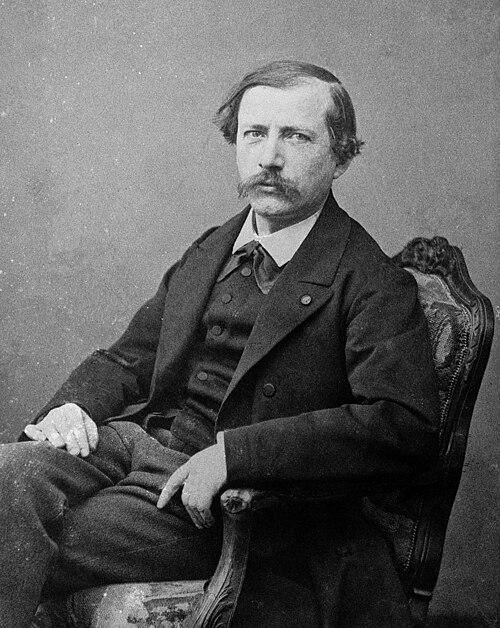
\includegraphics[width=\linewidth]{images/book3/berthelot.jpg}
\end{minipage}\hfill
\begin{minipage}[t]{0.76\linewidth}\vspace{0pt}
Marcellin Berthelot (1827--1907) verbrandde organische verbindingen in samengeperste
zuurstof in een gesloten, met platina bekleed stalen vat, zodat de
verbranding volledig was en niets ontsnapte: de calorimetrische bom, nog steeds
het referentie-instrument voor verbrandingswarmten. Hij bedacht ook de woorden
\omterm{def:b2:reaction-enthalpy:exothermic}{exotherm} en \omterm{def:b2:reaction-enthalpy:exothermic}{endotherm}. (Foto: publiek domein, Wikimedia
Commons.)
\end{minipage}
\end{history}

\section{Oefeningen}

\begin{exercise}[$\star$]\label{exo:b2:reaction-enthalpy:1}
Bereken met de standaardvormingsenthalpieën van het hoofdstuk
$\Delta_r H^\circ$ bij \qty{298}{K} van de verbranding van propaan,
\ce{C3H8(g) + 5O2(g) -> 3CO2(g) + 4H2O(l)}, gegeven $\Delta_f
H^\circ(\ce{C3H8}, \text{g}) = \qty{-104.7}{kJ/mol}$. Is de reactie
\omterm{def:b2:reaction-enthalpy:exothermic}{exotherm}?
% ledger: dfh:C3H8_g
\end{exercise}

\begin{exercise}[$\star$]\label{exo:b2:reaction-enthalpy:2}
Bereken de warmte die vrijkomt bij het verbranden van \qty{1.00}{kg} methaan (water
vloeibaar gevormd) en van \qty{1.00}{kg} diwaterstof, \ce{H2(g) + 1/2O2(g) ->
H2O(l)}. Welke brandstof levert meer warmte per kilogram?
\end{exercise}

\begin{exercise}[$\star$]\label{exo:b2:reaction-enthalpy:3}
Een bomcalorimeter geeft $\Delta_r U = \qty{-3264}{kJ/mol}$ voor vloeibaar
benzeen dat verbrandt volgens \ce{C6H6(l) + 15/2O2(g) -> 6CO2(g) + 3H2O(l)} bij
\qty{298}{K}. Bereken $\Delta_r H$.
\end{exercise}

\begin{exercise}[$\star$]\label{exo:b2:reaction-enthalpy:4}
Gegeven $\Delta_r H^\circ = \qty{-393.5}{kJ/mol}$ voor \ce{C(s) + O2(g) ->
CO2(g)} en $\Delta_r H^\circ = \qty{-283.0}{kJ/mol}$ voor \ce{CO(g) +
1/2O2(g) -> CO2(g)}. Bereken de enthalpie van \ce{CO2(g) + C(s) -> 2CO(g)},
de reactie die plaatsvindt in de hete cokes van een hoogoven.
\end{exercise}

\begin{exercise}[$\star\star$]\label{exo:b2:reaction-enthalpy:5}
Schat met de bindingsenthalpieën van het hoofdstuk de enthalpie van
\ce{CH4(g) + Cl2(g) -> CH3Cl(g) + HCl(g)}, met \qty{350}{kJ/mol} voor
C--Cl. Bereken daarna dezelfde grootheid uit de vormingsenthalpieën,
gegeven $\Delta_f H^\circ(\ce{CH3Cl}, \text{g}) = \qty{-83.7}{kJ/mol}$, en
becommentarieer het verschil.
% ledger: dfh:CH3Cl_g
\end{exercise}

\begin{exercise}[$\star\star$]\label{exo:b2:reaction-enthalpy:6}
De standaardverdampingsenthalpie van water bij \qty{298}{K} is
$\Delta_f H^\circ(\ce{H2O}, \text{g}) - \Delta_f H^\circ(\ce{H2O},
\text{l})$. Bereken ze. Schat ze met $C_{p,m}^\circ = \qty{75.35}{J/(K.mol)}$ voor
de vloeistof en \qty{33.59}{J/(K.mol)} voor de damp, beide constant
verondersteld, bij \qty{400}{K} (oververhit water onder druk),
en vergelijk met de tabellen, die $\Delta_f H^\circ =
\qty{-282.59}{kJ/mol}$ geven voor de vloeistof en \qty{-242.85}{kJ/mol} voor de
damp bij \qty{400}{K}.
% ledger: cp:H2O_l.298, cp:H2O_g.298, janafdfH:H2O_l.400, janafdfH:H2O_g.400
\end{exercise}

\begin{exercise}[$\star\star$]\label{exo:b2:reaction-enthalpy:7}
Bereken met een kringproces van Born--Haber de \omterm{def:b2:reaction-enthalpy:lattice-enthalpy}{roosterenthalpie} van
kaliumchloride uit: $\Delta_f H^\circ(\ce{KCl}, \text{s}) = \qty{-436.7}{kJ/mol}$,
sublimatie van kalium \qty{89.0}{kJ/mol}, ionisatie-energie van
kalium \qty{4.341}{eV}, $\Delta_f H^\circ(\ce{Cl}, \text{g}) =
\qty{121.3}{kJ/mol}$, elektronenaffiniteit van chloor \qty{3.613}{eV}. Waarom is
ze kleiner dan die van natriumchloride?
% ledger: dfh:KCl_cr, dfh:K_g, ie:K, janaf:Cl, ea:Cl
\end{exercise}

\begin{exercise}[$\star\star$]\label{exo:b2:reaction-enthalpy:8}
Een koffiebekercalorimeter wordt geijkt door er \qty{2.00}{kJ}
elektrische energie aan toe te voeren, wat zijn temperatuur met \qty{0.418}{K} doet stijgen. Daarna
wordt er \qty{50.0}{mL} zoutzuur van \qty{1.00}{mol/L} in gemengd
met \qty{50.0}{mL} natronloog van \qty{1.10}{mol/L},
beide bij dezelfde begintemperatuur: de temperatuur stijgt met
\qty{0.583}{K}. Bereken de enthalpie van \ce{H3O+(aq) + OH-(aq) ->
2H2O(l)}.
\end{exercise}

\begin{exercise}[$\star\star$]\label{exo:b2:reaction-enthalpy:9}
Octaan, een model voor benzine, heeft $\Delta_f H^\circ(\text{l}) =
\qty{-250.3}{kJ/mol}$. Bereken de enthalpie van zijn verbranding (water
vloeibaar), de warmte die per kilogram vrijkomt, en de massa koolstofdioxide
die per megajoule wordt uitgestoten. Vergelijk met methaan.
% ledger: dfh:C8H18
\end{exercise}

\begin{exercise}[$\star\star\star$]\label{exo:b2:reaction-enthalpy:10}
Bereken de \omterm{def:b2:reaction-enthalpy:flame-temperature}{adiabatische vlamtemperatuur} van methaan dat verbrandt in de
stoichiometrische hoeveelheid zuivere zuurstof, met constante warmtecapaciteiten (die
van het hoofdstuk bij \qty{298}{K}: \ce{CO2} 37.13, \ce{H2O(g)}
\qty{33.59}{J/(K.mol)}). Vergelijk met het resultaat in lucht,
\qty{2780}{K} in dezelfde benadering. Waarom is de werkelijke vlam in zuurstof
veel kouder dan deze berekening zegt?
% ledger: cp:CO2_g.298, cp:H2O_g.298
\end{exercise}

\begin{exercise}[$\star\star\star$]\label{exo:b2:reaction-enthalpy:11}
De warmtecapaciteit van een gas wordt vaak geschreven als $C_{p,m}^\circ = a + bT$. Neem voor
de ammoniaksynthese $\Delta_r a = \qty{-60.5}{J/(K.mol)}$ en
$\Delta_r b = \qty{0.0540}{J/(K^2.mol)}$ (aangepast aan de tabellen tussen
\qty{300}{K} en \qty{800}{K}). Integreer de \omterm{thm:b2:reaction-enthalpy:kirchhoff}{wet van Kirchhoff} van
\qty{298}{K} tot \qty{700}{K} en vergelijk met de waarde uit de tabellen,
\qty{-105.2}{kJ/mol}, en met de schatting bij constante $C_p$.
\end{exercise}

\begin{exercise}[$\star\star\star$]\label{exo:b2:reaction-enthalpy:12}
Stikstofmonoxide ontstaat in motoren volgens \ce{N2(g) + O2(g) -> 2NO(g)}.
Bereken zijn \omterm{def:b2:reaction-enthalpy:standard-reaction-enthalpy}{standaardreactie-enthalpie} bij \qty{298}{K}. Toon aan dat de reactie,
als $\Delta_r C_p^\circ$ klein is, bij \qty{2000}{K} ongeveer evenveel warmte
opneemt; schat met de warmtecapaciteiten van de tabellen bij \qty{298}{K}
(\ce{NO} \qty{29.85}{J/(K.mol)}, \ce{N2} 29.12, \ce{O2}
\qty{29.38}{J/(K.mol)}) de verandering tussen
\qty{298}{K} en \qty{2000}{K}. Leg uit waarom een \omterm{def:b2:reaction-enthalpy:exothermic}{endotherme} reactie juist
in de heetste vlammen een probleem kan zijn.
% ledger: dfh:NO_g, cp:NO_g.298, cp:N2_g.298, cp:O2_g.298
\end{exercise}

\section{Probleem: het kampeergaspatroon}

\begin{problem}[{Weekendprobleem --- de energie van butaan, een meting in
een bomcalorimeter, het water dat in een pan wordt verwarmd, en de temperatuur van de
vlam}]
\label{pb:b2:reaction-enthalpy:1}
Een kampeerbrander verbrandt butaan uit een patroon met \qty{230}{g} inhoud.
Gegevens bij \qty{298}{K} ($\Delta_f H^\circ$ in \unit{kJ/mol}): \ce{C4H10(g)}
$-125.6$, \ce{CO2(g)} $-393.51$, \ce{H2O(l)} $-285.83$, \ce{H2O(g)}
$-241.83$. Molaire massa's: \ce{C4H10} \qty{58.12}{g/mol}, \ce{H2O}
\qty{18.02}{g/mol}. Warmtecapaciteit van vloeibaar water
\qty{75.35}{J/(K.mol)}. Droge lucht: \qty{20.95}{\percent} \ce{O2},
\qty{78.08}{\percent} \ce{N2}, \qty{0.93}{\percent} \ce{Ar} in volume. $R = \qty{8.314}{J/(K.mol)}$.
% ledger: dfh:C4H10_g, dfh:CO2, dfh:H2O-l, dfh:H2O_g, cp:H2O_l.298, air:O2, air:N2, air:Ar

\medskip
\noindent\textbf{Deel I --- De brandstof.}
\begin{enumerate}
  \item Schrijf de volledige verbranding van butaan op, met vloeibaar gevormd water,
        voor één mol butaan.
  \item Bereken de \omterm{def:b2:reaction-enthalpy:standard-reaction-enthalpy}{standaardreactie-enthalpie} ervan bij \qty{298}{K}.
  \item Bereken ze opnieuw met het water als damp gevormd, en verklaar het
        verschil.
  \item Bereken in beide gevallen de warmte die per gram butaan vrijkomt.
  \item Welke van de twee waarden beschrijft een kampeerbrander, waarvan het water
        de vlam als damp verlaat?
  \item Hoeveel warmte kan het hele patroon op de brander vrijgeven?
\end{enumerate}

\medskip
\noindent\textbf{Deel II --- Een meting.}
Een monster van \qty{0.500}{g} butaan wordt verbrand in een bomcalorimeter met een
warmtecapaciteit van \qty{10.00}{kJ/K}; het gevormde water condenseert.
\begin{enumerate}[resume]
  \item Welke grootheid meet een bomcalorimeter, en waarom?
  \item Bereken $\Delta\nu_{\text{gas}}$ van de reactie van vraag 1.
  \item Bereken de verwachte $\Delta_r U$.
  \item Bereken de verwachte temperatuurstijging van de calorimeter.
  \item De afgelezen stijging is \qty{2.461}{K}. Leid de gemeten $\Delta_r U$
        en $\Delta_r H$ af, en het relatieve verschil met de tabellen.
\end{enumerate}

\medskip
\noindent\textbf{Deel III --- De pan.}
\begin{enumerate}[resume]
  \item Bereken de warmte die nodig is om \qty{1.00}{L} water
        (\qty{1.00}{kg}) van \qty{20}{\celsius} tot \qty{100}{\celsius} te brengen.
  \item De brander doet dat met \qty{16.0}{g} butaan. Bereken zijn
        rendement (door het water opgenomen warmte gedeeld door vrijgekomen warmte).
  \item Waar blijft de rest van de warmte?
  \item Hoeveel liter water kan het hele patroon bij dit rendement aan de kook
        brengen?
\end{enumerate}

\medskip
\noindent\textbf{Deel IV --- De vlam.}
\begin{enumerate}[resume]
  \item Butaan verbrandt in de stoichiometrische hoeveelheid lucht. Bereken de
        hoeveelheden distikstof en argon die meekomen met de dizuurstof die
        één mol butaan nodig heeft.
  \item Geef de hoeveelheden van de producten, stikstof en argon inbegrepen.
  \item Leg met een weg in twee stappen uit waarom de warmte die de reactie bij
        \qty{298}{K} vrijgeeft (water als damp) volledig wordt gebruikt om
        deze gassen op te warmen.
  \item Bereken met de warmtecapaciteiten bij \qty{298}{K}, \ce{CO2} 37.13,
        \ce{H2O(g)} 33.59, \ce{N2} 29.12, \ce{Ar} \qty{20.79}{J/(K.mol)},
        de warmtecapaciteit van de producten.
  \item Leid de vlamtemperatuur af bij constante warmtecapaciteiten.
  \item De enthalpietoenamen uit de tabellen geven, voor de producten van één
        mol butaan, \qty{2515.7}{kJ} tussen \qty{298}{K} en
        \qty{2300}{K}, en \qty{2655.7}{kJ} tussen \qty{298}{K} en
        \qty{2400}{K}. Bepaal de vlamtemperatuur door lineaire interpolatie.
  \item Waarom is de eerste schatting te hoog?
  \item Waarom is de gemeten temperatuur van een butaanvlam nog lager?
  \item Geef de \omterm{def:b2:reaction-enthalpy:flame-temperature}{adiabatische vlamtemperatuur} van butaan in lucht.
\end{enumerate}
\end{problem}
